\documentclass{beamer}
\mode<presentation>
\usepackage{amsmath,amssymb,mathtools}
\usepackage{listings}
\usepackage{graphicx}
\usetheme{Boadilla}
\usecolortheme{lily}
\setbeamertemplate{footline}{
  \leavevmode%
  \hbox{%
  \begin{beamercolorbox}[wd=\paperwidth,ht=2ex,dp=1ex,right]{author in head/foot}%
    \insertframenumber{} / \inserttotalframenumber\hspace*{2ex}
  \end{beamercolorbox}}%
  \vskip0pt%
}
\setbeamertemplate{navigation symbols}{}
\lstset{
  frame=single,
  breaklines=true,
  columns=fullflexible,
  basicstyle=\ttfamily\tiny
}
\providecommand{\abs}[1]{\left\vert#1\right\vert}
\let\vec\mathbf
\title{Discrete -- Problem 1.2.56}
\author{ee25btech11056 -- Suraj.N}
\begin{document}
\begin{frame}
  \titlepage
\end{frame}
\begin{frame}{Problem Statement}
The iteration $x_{n+1} = \dfrac{1}{1 + x_n^2}$ converges to a real number $x$ in the
interval $(0,1)$ with $x_0 = 0.5$. The value of $x$ correct up to 2 decimal places is:

\begin{enumerate}
\item a) $0.65$
\item b) $0.68$
\item c) $0.73$
\item d) $0.80$
\end{enumerate}
\end{frame}
\begin{frame}{Key Concept: Fixed-Point Iteration}
A fixed point of a function $g(x)$ is a value $x^*$ such that
\[
  g(x^*) = x^*.
\]
The iteration $x_{n+1} = g(x_n)$ converges to $x^*$ if the contraction condition holds:
\[
  \abs{g'(x^*)} < 1.
\]
Here $g(x) = \dfrac{1}{1+x^2}$, so we seek $x^* \in (0,1)$ satisfying
\[
  x^* = \frac{1}{1+(x^*)^2}.
\]
\end{frame}

\begin{frame}{Applying MVT to the Iteration Error}
Define the \textbf{error} at step $n$:
\[
  e_n = x_n - x^*
\]
This measures how far you currently are from the answer.

Apply MVT to $g$ between $x_n$ and $x^*$:
\[
  g(x_n) - g(x^*) = g'(c)\cdot(x_n - x^*) \quad \text{for some } c
  \text{ between } x_n \text{ and } x^*
\]
Now substitute what you know:
\begin{enumerate}
\item Left side: $g(x_n) = x_{n+1}$ and $g(x^*) = x^*$, so left side $= e_{n+1}$
\item Right side: $(x_n - x^*) = e_n$
\end{enumerate}
This gives the key result:
\[
\boxed{e_{n+1} = g'(c)\cdot e_n}
\]
\textbf{The error at the next step equals the current error multiplied by $g'(c)$.}\\ 
Therefore , $\abs{g'(x^*)} < 1 \Rightarrow$ error shrinks every step $\Rightarrow$ \textbf{converges}
\end{frame}

\begin{frame}{Setting Up the Fixed-Point Equation}
Multiply both sides by $1+(x^*)^2$:
\[
  x^*\bigl(1+(x^*)^2\bigr) = 1.
\]
Expanding:
\[
  (x^*)^3 + x^* - 1 = 0.
\]
Let $f(x) = x^3 + x - 1$. We locate the root:
\begin{enumerate}
\item $f(0) = -1 < 0$
\item $f(1) = 1 > 0$
\end{enumerate}
By the Intermediate Value Theorem, a root exists in $(0,1)$.
\end{frame}
\begin{frame}{Verifying the Contraction Condition}
Compute the derivative of $g(x)$:
\[
  g'(x) = \frac{-2x}{(1+x^2)^2}.
\]
At $x^* \approx 0.68$:
\[
  g'(0.68) = \frac{-2(0.68)}{(1+(0.68)^2)^2}
           = \frac{-1.36}{(1.4624)^2}
           \approx \frac{-1.36}{2.139}
           \approx -0.636.
\]
Since $\abs{g'(x^*)} \approx 0.636 < 1$, the contraction condition is satisfied and the iteration \textbf{converges}.
\end{frame}

\begin{frame}{Solving the given equation}

Solve:
\[
x^3 + x - 1 = 0
\]

This is in standard cubic form:
\[
x^3 + px + q = 0
\]

Comparing:
\[
p = 1, \quad q = -1
\]

Using Cardano formula for equation:
\[
x^3 + px + q = 0
\]

Solution:
\[
x = \sqrt[3]{-\frac{q}{2} + \sqrt{D}} + \sqrt[3]{-\frac{q}{2} - \sqrt{D}}
\]

where discriminant:
\[
D = \left(\frac{q}{2}\right)^2 + \left(\frac{p}{3}\right)^3
\]

\end{frame}

%------------------------------------------------

\begin{frame}

Calculating the discriminant
\[
D = \left(\frac{-1}{2}\right)^2 + \left(\frac{1}{3}\right)^3
\]

\[
D = \frac{1}{4} + \frac{1}{27}
\]

\[
D = \frac{27 + 4}{108} = \frac{31}{108}
\]

Substituting the value of the discriminant to find x : 
\[
x = \sqrt[3]{\frac{1}{2} + \sqrt{\frac{31}{108}}}
+
\sqrt[3]{\frac{1}{2} - \sqrt{\frac{31}{108}}}
\]
\[
x = \sqrt[3]{0.5 + 0.536} + \sqrt[3]{0.5 - 0.536}
\]

\[
x = \sqrt[3]{1.036} + \sqrt[3]{-0.036}
\]

\[
x \approx 1.012 - 0.33 = 0.68
\]

\end{frame}



\begin{frame}{Conclusion}
The fixed-point iteration $x_{n+1} = \dfrac{1}{1+x_n^2}$ with $x_0 = 0.5$ converges to the
unique root of
\[
  x^3 + x - 1 = 0 \quad \text{in } (0,1).
\]
The converged value correct to 2 decimal places is
\[
  x^* \approx 0.68.
\]
The correct answer is \textbf{b) 0.68}.
\end{frame}

\begin{frame}{Plot of Sequence} 

\begin{figure}[h!]
  \centering
  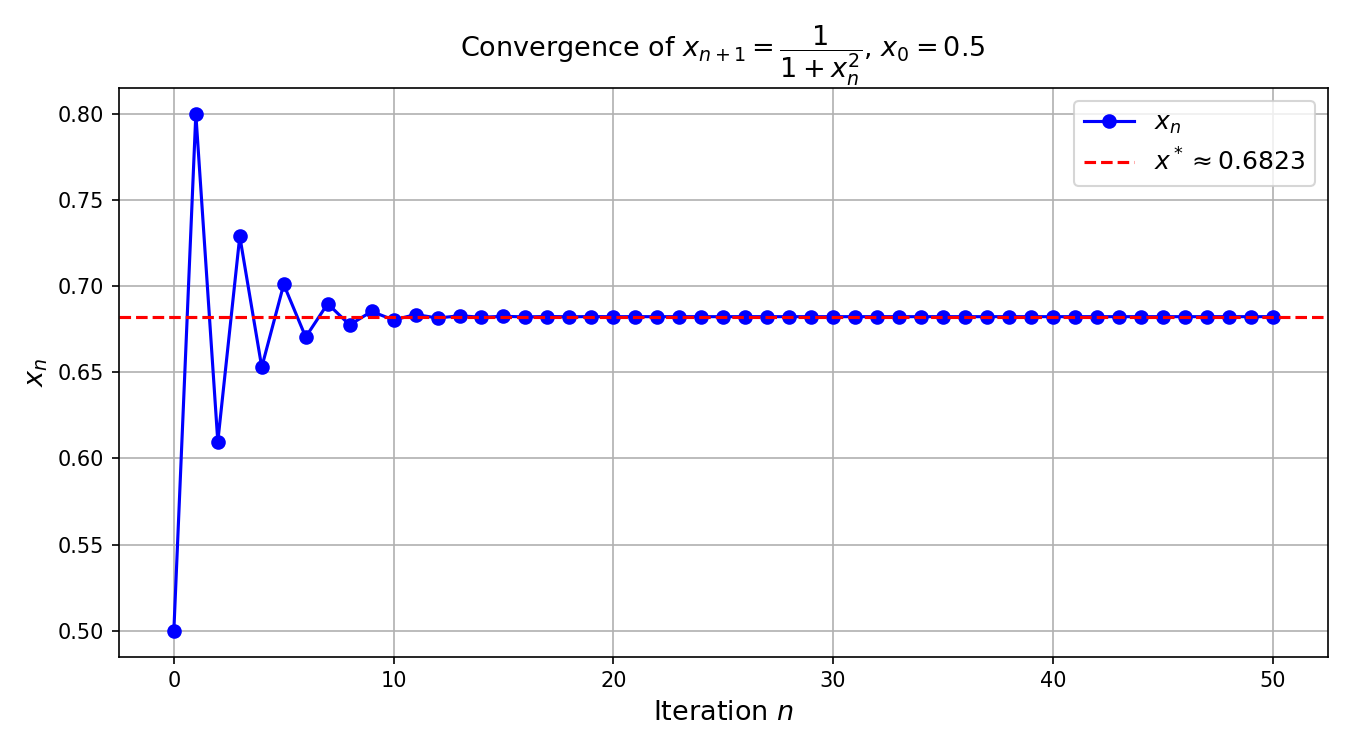
\includegraphics[width=1\columnwidth]{figs/convergence_plot.png} 
  \caption{Sequence}
  \label{Fig1}
\end{figure}


\end{frame}


\begin{frame}[fragile]{Python Code: Convergence Value}
\begin{lstlisting}[language=Python]
def g(x):
    return 1.0 / (1.0 + x**2)

x = 0.5
tol = 1e-10
max_iter = 1000
x_new = x

for i in range(max_iter):
    x_new = g(x)
    print(f"The {i} iteration value is : {x_new}")
    if abs(x_new - x) < tol:
        print(f"Converged at iteration {i+1}")
        break
    x = x_new

print(f"Fixed point x* = {x_new:.10f}")
print(f"Rounded to 2 decimal places = {round(x_new, 2)}")

# Verification: solve x^3 + x - 1 = 0
import numpy as np
roots = np.roots([1, 0, 1, -1])
real_roots = [r.real for r in roots if abs(r.imag) < 1e-10]
print(f"Root of x^3+x-1=0 in (0,1): {real_roots[0]:.10f}")
\end{lstlisting}
\end{frame}
\begin{frame}[fragile]{Python Code: Convergence Plot}
\begin{lstlisting}[language=Python]
import numpy as np
import matplotlib.pyplot as plt

def g(x):
    return 1.0 / (1.0 + x**2)
x = 0.5
iterates = [x]
tol = 1e-10
max_iter = 50
for i in range(max_iter):
    x_new = g(x)
    iterates.append(x_new)
    if abs(x_new - x) < tol:
        print(f"Converged at iteration {i+1}")
        break
    x = x_new
x_star = iterates[-1]
n_vals = list(range(len(iterates)))

plt.figure(figsize=(9, 5))
plt.plot(n_vals, iterates, 'bo-', markersize=6,
         linewidth=1.5, label=r'$x_n$')
plt.axhline(y=x_star, color='r', linestyle='--',
            linewidth=1.5, label=f'x* = {x_star:.4f}')
plt.xlabel('Iteration n', fontsize=13)
plt.ylabel('x_n', fontsize=13)
plt.title('Convergence of Fixed-Point Iteration', fontsize=13)
plt.legend(fontsize=12)
plt.grid(True)
plt.tight_layout()
plt.savefig('convergence_plot.png', dpi=150)
plt.show()
\end{lstlisting}
\end{frame}
\end{document}
